\chapter{Trajectory pre-processing}
\label{ch:preproc}

The pre-processing turns each IGC file into a trajectory fit for analysis. This
chapter covers its first five steps, in the order they run: reading the fixes,
choosing the altitude channel, deleting fixes with a stale clock or a repeated
position, and dropping tracks that are too fast.

\section{Reading the fixes}
\label{sec:parsing}

Each \texttt{B} record gives a fix $(t_i,\varphi_i,\lambda_i)$, with latitude and
longitude in degrees, together with the validity flag and the two altitudes
$h_i^{\mathrm{baro}}$ and $h_i^{\mathrm{GNSS}}$. A record that does not follow the
fixed layout of the format, or whose time of day or position is impossible, is
discarded. A missing or unreadable altitude,
including the zero the format uses for a missing reading, is marked as missing, and
the fix keeps its time and position.

Time is measured in seconds from the first fix. Records carry only the time of day,
so a flight crossing UTC midnight would jump back by a day; a day is added when the
clock passes from the last hour of one day to the first hour of the next. Other
backward steps and repeated times are left to the clock rule of
Section~\ref{sec:clock}. Well-formed but implausible fixes, such as position spikes,
are kept as well: the parser discards only what cannot be read. The validity flag, which marks
fixes without a three-dimensional GNSS solution, is kept but not used at this stage.

\section{Choice of altitude channel}
\label{sec:altchannel}

Some recorders log no pressure altitude, so we use GNSS altitude for every flight,
$z=h^{\mathrm{GNSS}}$. Its vertical datum is not uniform across recorders: the IGC
specification prescribes height above the WGS84 ellipsoid~\cite{fai_igc_spec}, the
CIVL specification for hang gliders and paragliders height above the
geoid~\cite{fai_civl_s7h_2024}. A constant offset cancels in altitude increments, but
comparing absolute altitudes across flights would need a datum audit.

Let $N$ be the number of fixes read from the file, before any is deleted, and $P$ the
set of those with a GNSS altitude. The flight is kept only if
\begin{equation}
  \frac{|P|}{N}\geq\cfgAltitudeGnssPresentMin
  \qquad\text{and}\qquad
  \max_{i\in P}h_i^{\mathrm{GNSS}}-\min_{i\in P}h_i^{\mathrm{GNSS}}\geq\SI{\cfgAltitudeGnssMinRangeM}{\metre}.
  \label{eq:gnss-admission}
\end{equation}
The first condition rejects incomplete channels; the second rejects channels stuck at
one value, and flights with almost no vertical excursion. Fixes flagged as lacking a
three-dimensional solution count as present if they carry an altitude. Pressure
altitude is never substituted for a missing GNSS value.

The barometer is checked with the same two conditions on $h^{\mathrm{baro}}$, with
thresholds \cfgAltitudeBaroWitnessPresentMin\ and
\SI{\cfgAltitudeBaroWitnessMinRangeM}{\metre}. A flight whose
barometer passes is marked, so that later cleaning steps can use pressure altitude as
independent evidence; the mark does not decide whether the flight is kept.

\section{Clock}
\label{sec:clock}

% To write. Code: clean.increasing_time, on the fixes as read (step 2 deletes none).
% Fix i is kept iff t_i > max_{j<i} t_j. A repeated second keeps its first fix; a
% backward step is deleted, with every fix after it until the clock passes the latest
% time kept. Afterwards the times are strictly increasing (needed in Sec. fasttracks).

\section{Repeated positions}
\label{sec:repeated}

% To write. Code: clean.moving_position, on the fixes the clock rule left.
% Fix i is deleted iff lat_i = lat_{i-1} and lon_i = lon_{i-1}, exactly (same IGC
% digits); altitude is not compared. In a run of identical positions only the first
% fix stays. Reason: the recorder repeats its last position while the clock runs.

\section{Fast tracks}
\label{sec:fasttracks}

% To write. Code: speed.step_speed and speed.track_speed, on the fixes left by the
% two rules above. Step speed v_i = 3.6 d_i / (t_{i+1} - t_i) in km/h, d_i the
% haversine distance between fixes i and i+1 on a sphere of radius 6371 km. The
% flight is kept iff the median of its v_i is <= the threshold (or it has no step).
% The figures plot that median, one value per flight: write v_i and the median as
% equations. The threshold max_kmh (single steps) belongs to the excursion rule.

\begin{figure}[htbp]
\centering
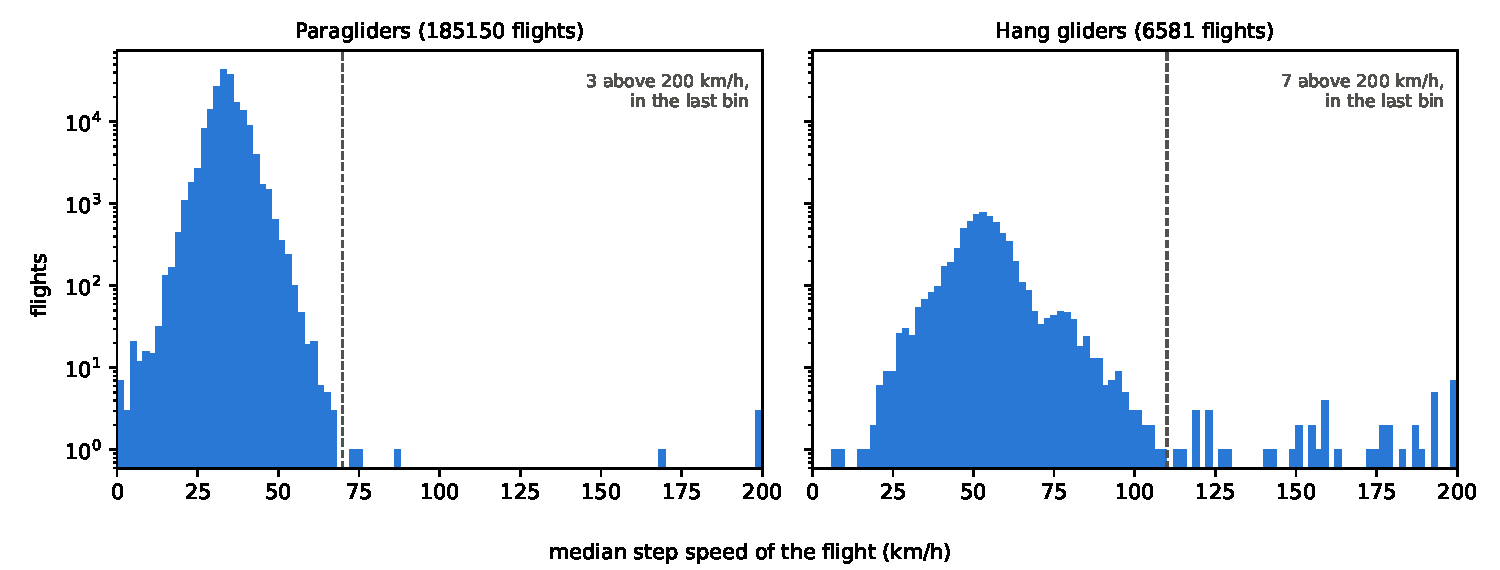
\includegraphics[width=\textwidth]{generated/figures/preprocessing/median-speed}
\caption{Median step speed of every flight past the altitude channel, computed on
the fixes left by the clock and repeated-position rules, in bins of 2~km/h on a
logarithmic scale. Flights above 200~km/h are counted in the last bin. The dashed
line marks the threshold,
\SI[per-mode=symbol]{\cfgSpeedMedianMaxKmhPara}{\kilo\metre\per\hour} for
paragliders and
\SI[per-mode=symbol]{\cfgSpeedMedianMaxKmhHang}{\kilo\metre\per\hour} for hang
gliders.}
\label{fig:median-speed}
\end{figure}

\begin{figure}[htbp]
\centering
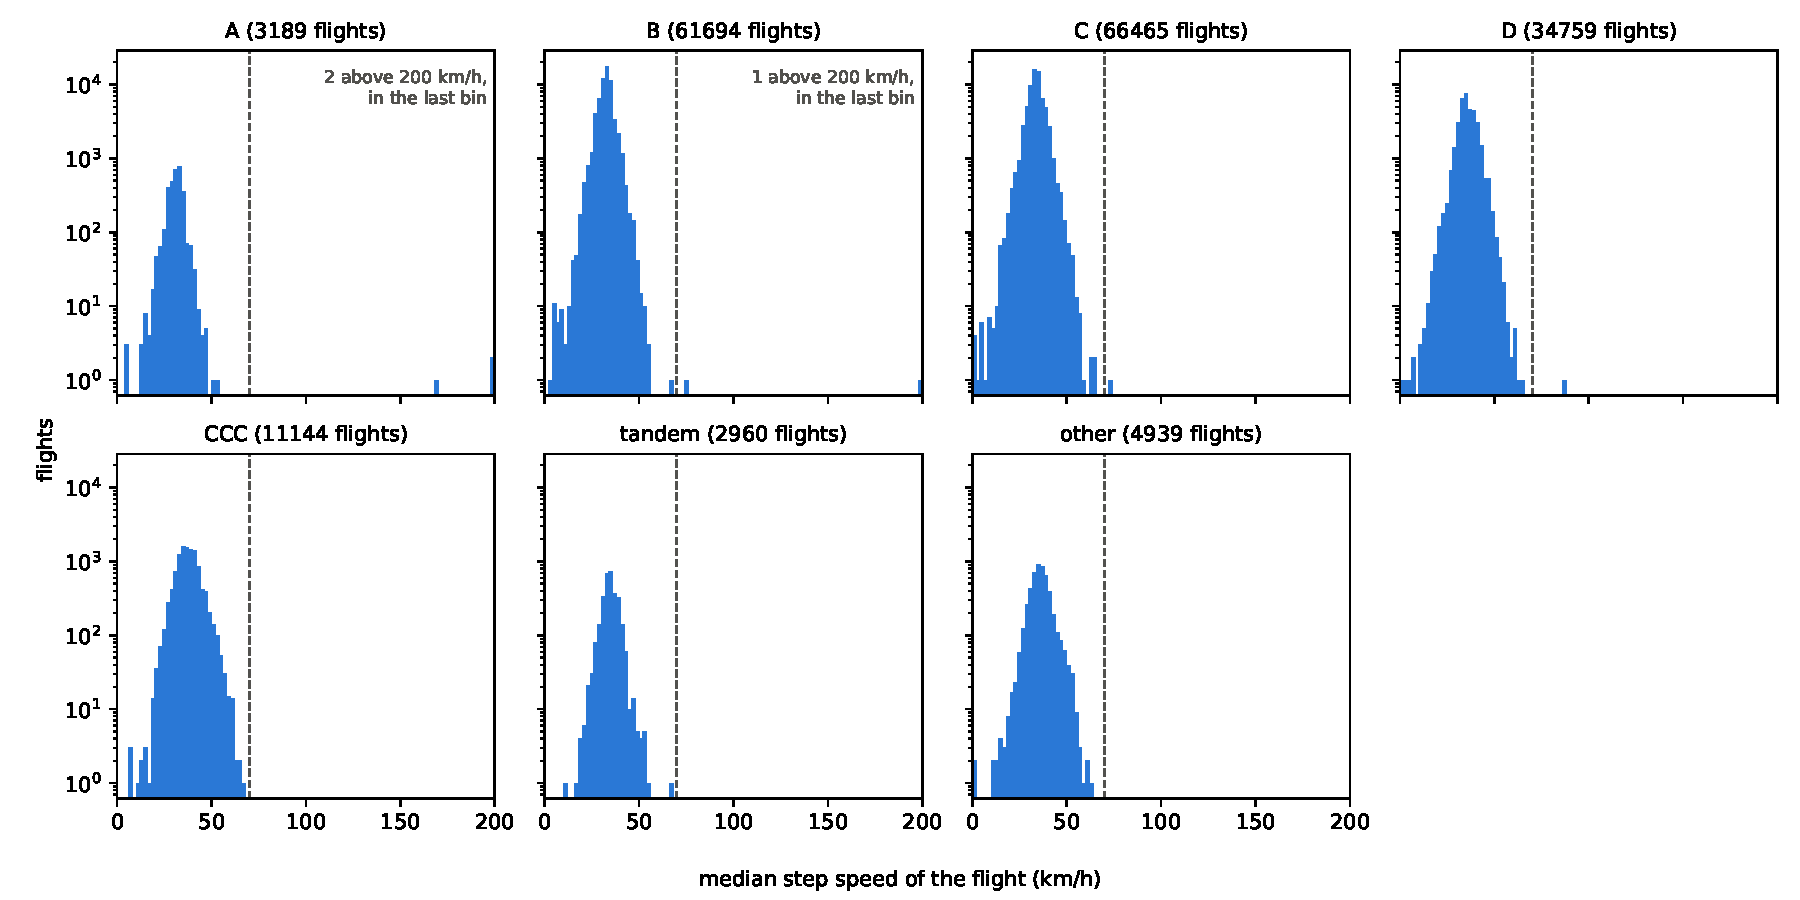
\includegraphics[width=\textwidth]{generated/figures/preprocessing/median-speed-para-classes}
\caption{As Figure~\ref{fig:median-speed}, for paragliders by wing class
(Section~\ref{sec:glider}): EN classes A to D, the CIVL Competition Class (CCC),
tandem wings, certified or not, and every other label.}
\label{fig:median-speed-para-classes}
\end{figure}

\begin{figure}[htbp]
\centering
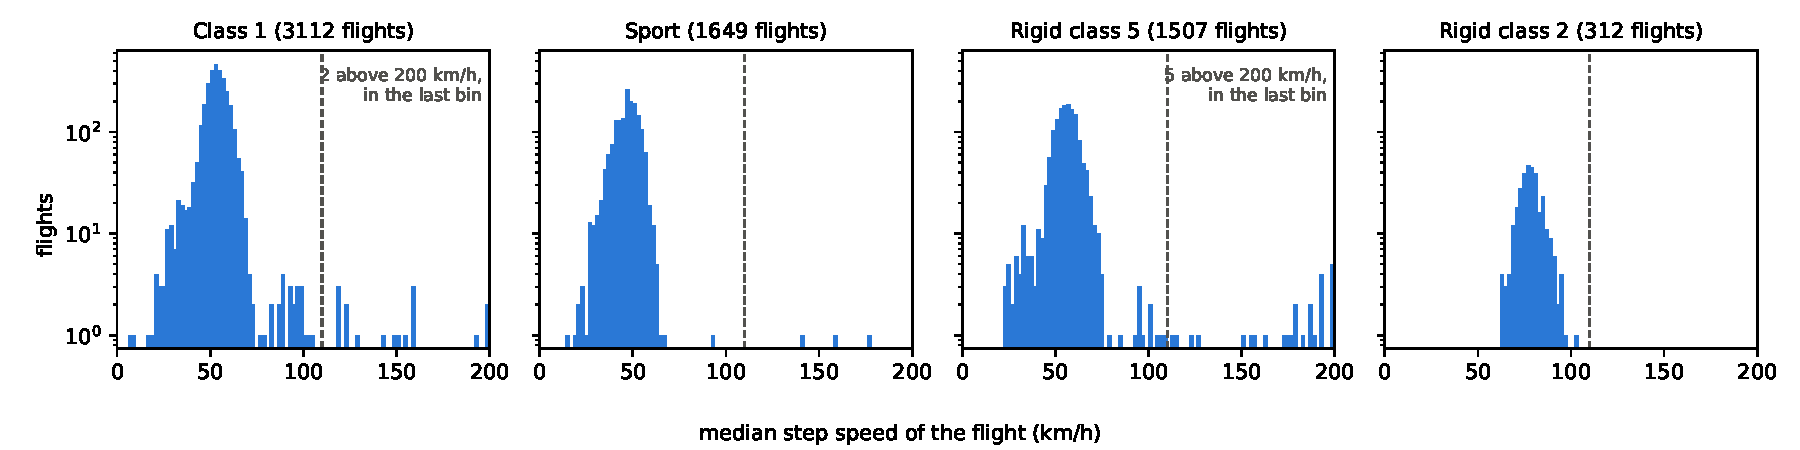
\includegraphics[width=\textwidth]{generated/figures/preprocessing/median-speed-hang-classes}
\caption{As Figure~\ref{fig:median-speed}, for hang gliders by wing class
(Section~\ref{sec:glider}): Class~1, its Sport sub-class, and the rigid Classes~5
and~2. Flights of any other class are not shown.}
\label{fig:median-speed-hang-classes}
\end{figure}
